% Provenance (never printed): see sources/outline_sources.md (Year 1: morphology,
% gravity, heat flow and seismicity of a subduction zone; accretionary and erosive
% margins; slab geometry; volcanic arcs). Kuril map, section and numbers from
% figdata/bachelor-1/slab_seismicity.py; exercise and problem values in the Book 3
% scratch calculator calc/ch14.py.
\chapter{الهوامش النشطة}\label{ch:b1:active-margins}

في 11 مارس 2011، عند الساعة 14:46 بالتوقيت المحلي، انكسر حدّ الصفيحة قبالة شمال شرق اليابان على امتداد نحو \qty{400}{km} على طول الخندق، وعلى عمق \qty{150}{km} تحت انحداره. وانزلق الصدع بما يصل إلى 50 إلى \qty{60}{m}، معظمه صاعدًا على \omterm{def:b1:geological-maps:attitude}{الانحدار} من البؤرة نحو خندق اليابان؛ وعلى اليابسة تحرّك الساحل أفقيًا وهبط. والصفيحة التي تغوص هناك، صفيحة المحيط الهادئ، تنزل تحت اليابان على سطح تحدّده الزلازل حتى مئات الكيلومترات؛ وحيث يقع ذلك السطح على عمق نحو مائة كيلومتر، يمتد خط من البراكين موازيًا للساحل. يقرأ هذا الفصل مثل هذا الهامش من شكله، ومن جاذبيته، ومن تدفّقه الحراري، وقبل كل شيء من زلازله.
% ledger: usgs:tohoku, wada:decoupling

\begin{recall}
يعود \omterm{def:b1:layered-earth:lithosphere}{الغلاف الصخري} المحيطي إلى \omterm{def:b1:layered-earth:layers}{الوشاح} عند مناطق الاندساس، وتُعلَّم بالخنادق وبأحزمة مائلة من الزلازل، \omterm{def:b1:layered-earth:lithosphere}{والغلاف الصخري} القديم يغوص تحت وزنه (الكتاب 2، الصف 11)؛ والماء المنبعث من الصفيحة الغائصة يخفض درجة حرارة انصهار \omterm{def:b1:layered-earth:layers}{الوشاح} فوقها (الكتاب 2، الصف 12). وتنتشر الحرارة على مسافة $L$ في زمن من رتبة $L^2/\kappa$ (\cref{ch:b1:heat-budget})؛ وصفيحة لا نهائية كثافتها $\rho$ وسمكها $h$ تجذب بمقدار $2\pi G\rho h$ (\cref{ch:b1:isostasy-gravity})؛ وتدور الصفائح حول أقطاب أويلر (\cref{ch:b1:plate-kinematics})؛ ويتناقص التدفّق الحراري لقاع المحيط كجذر مقلوب لعمره (\cref{ch:b1:rifts-ridges-margins}).
\end{recall}

\section{تشريح الهامش النشط}\label{sec:b1:active-margins:anatomy}

\begin{definition}[الهامش النشط؛ الخندق المحيطي؛ المنطقة الأمامية للقوس؛ حوض خلف القوس]\label{def:b1:active-margins:active-margin}
\emph{الهامش النشط}\index{الهامش النشط} حدّ صفيحتين متقاربتين تغوص عنده \omterm{def:b1:layered-earth:lithosphere}{الغلاف الصخري} المحيطي تحت صفيحة أخرى، إما تحت قارة أو تحت صفيحة محيطية أخرى. و\emph{الخندق المحيطي}\index{الخندق المحيطي} منخفض طويل ضيّق على شكل حرف V في قاع البحر، تنحني الصفيحة الغائصة على طوله نازلةً تحت الأخرى. و\emph{المنطقة الأمامية للقوس}\index{المنطقة الأمامية للقوس} هي الجزء من الصفيحة المتراكبة بين الخندق وخط البراكين. و\emph{حوض خلف القوس}\index{حوض خلف القوس} حوض وراء البراكين، على الجانب البعيد عن الخندق، حيث تتمدّد الصفيحة المتراكبة وقد يتكوّن فيه \omterm{def:b1:layered-earth:layers}{قشرة} محيطية جديدة.
\end{definition}

الخنادق أعمق أماكن المحيطات، وأعمقها جميعًا هي هاوية تشالنجر في خندق ماريانا. وعبر خندق كوريل ينخفض القاع من نحو \qty{5200}{m} على السهل القاعي إلى \qty{8700}{m} عند المحور، أي أخفض بنحو \qty{3.5}{km}، والخندق لا يتجاوز عرضه عشرات الكيلومترات (الشكل في \cref{sec:b1:active-margins:gravity-heat}). وتبلغ الهوامش المتقاربة على الأرض نحو \qty{55000}{km} في المجموع؛ وفي نموذج رقمي لحدود الصفائح تبلغ حدود الاندساس نحو \qty{51000}{km}، مقابل نحو \qty{67000}{km} من الحيود الانتشارية.
% ledger: data:b3-grav-kuril (trench_gravity.py values), stern:subduction, data:pb2002 (ridge_budget.py)

على الجانب البحري للخندق ترتفع الصفيحة قليلًا قبل أن تنغمس، في رفعة خارجية عريضة منخفضة. وهناك تنحني الصفيحة ويتمدّد جزؤها العلوي: فزلازل الصدع العادي تصيب الرفعات الخارجية. ويطابق عرض الرفعة الخارجية انحناءَ صفيحة مرنة؛ وهذا الانحناء في \omterm{def:b1:layered-earth:lithosphere}{الغلاف الصخري} يُدرس في الكتاب 5. أما الخندق نفسه فهو المكان الذي يسحب فيه ثقل الصفيحة الغائصة الكثيفة حافتها الأمامية إلى الأسفل.

\begin{definition}[الكتلة المندسّة]\label{def:b1:active-margins:slab}
\emph{الكتلة المندسّة}\index{الكتلة المندسّة} هي الجزء من الصفيحة الغائصة الذي نزل بالفعل إلى \omterm{def:b1:layered-earth:layers}{الوشاح}: صفيحة من \omterm{def:b1:layered-earth:lithosphere}{الغلاف الصخري} المحيطي، تعلوها قشرتها، مائلة تحت الصفيحة المتراكبة من الخندق إلى أعماق تبلغ مئات الكيلومترات.
\end{definition}

تُقطَّع الصفيحة المتراكبة إلى شرائط موازية للخندق (الشكل أدناه): \omterm{def:b1:active-margins:active-margin}{المنطقة الأمامية للقوس}، وغالبًا معها كومة من الرواسب المكشوطة عند مقدّمتها وحوض رسوبي خلفها؛ \omterm{def:b1:active-margins:volcanic-arc}{والقوس البركاني}؛ وخلف بعض الأقواس، \omterm{def:b1:active-margins:active-margin}{حوض خلف القوس} وقوس قديم منقرض وراءه. وبين \omterm{def:b1:active-margins:slab}{الكتلة المندسّة} والصفيحة المتراكبة يقع إسفين من \omterm{def:b1:layered-earth:layers}{الوشاح}، يُسحب إلى الأسفل على طول أعلى الكتلة.

\begin{omfigure}
\begin{tikzpicture}[x=0.01667cm, y=0.01667cm, font=\scriptsize,
  lbl/.style={fill=white, fill opacity=0.8, text opacity=1, inner sep=1pt}]
\begin{scope}
\clip (-150,-330) rectangle (650,55);
% mantle and sea water
\fill[orange!12] (-150,-330) rectangle (650,15);
\fill[omSea!45] (-150,15) rectangle (650,0);
% incoming plate and slab: top dips 25 deg to 50 km, then 45 deg; 100 km thick
\fill[omLithBasalt!55] (-150,4) -- (-80,4) .. controls (-60,7) and (-40,7) .. (-25,4) -- (0,0)
  -- (107.2,-50) -- (420,-363) -- (349,-434) -- (48.9,-133.1) -- (-22.1,-100) -- (-150,-100) -- cycle;
\draw[omSea!50!black, line width=1.6pt] (-150,4) -- (-80,4) .. controls (-60,7) and (-40,7) .. (-25,4) -- (0,0) -- (107.2,-50) -- (420,-363);
% overriding plate
\fill[brown!28] (0,0) -- (12,3) -- (45,8) -- (60,10) -- (140,10) -- (150,12) -- (184,12) -- (230,9)
  -- (300,7) -- (395,6) -- (410,3) -- (420,2) -- (430,3) -- (445,6) -- (540,7) -- (560,14) -- (590,14)
  -- (610,10) -- (650,10) -- (650,-60) -- (520,-55) -- (445,-25) -- (420,-15) -- (395,-25) -- (320,-55)
  -- (250,-60) -- (117.2,-60) -- (107.2,-50) -- cycle;
% accretionary prism and forearc basin
\fill[yellow!55] (0,0) -- (12,3) -- (45,8) -- (60,10) -- (60,-28) -- cycle;
\draw[black!45, line width=0.3pt] (14,-3) -- (24,5) (28,-7) -- (38,6) (42,-14) -- (52,8);
\fill[yellow!30] (68,10) -- (132,10) -- (122,4) -- (78,4) -- cycle;
% arc volcano
\fill[black!60] (150,12) -- (167,26) -- (184,12) -- cycle;
% an isotherm: a cold tongue down the slab
\draw[omDef, dashed, line width=0.6pt] (-150,-82) -- (-30,-82) -- (40,-118) -- (300,-318)
  -- (232,-200) -- (150,-112) .. controls (130,-80) and (180,-72) .. (260,-72) -- (650,-72);
% mantle wedge flow
\draw[->, black!60, line width=0.5pt] (600,-130) .. controls (450,-135) and (300,-125) .. (215,-150)
  .. controls (205,-160) and (240,-185) .. (300,-235);
% water and melt
\foreach \x/\z in {150/-93, 172/-115, 194/-137}
  \draw[->, blue!70!black, line width=0.5pt] (\x,\z) -- (\x-6,\z+28);
\draw[red!75!black, line width=0.8pt, decorate, decoration={snake, amplitude=1.2, segment length=6}] (167,-100) -- (167,12);
% earthquakes
\foreach \x/\z in {20/-12, 45/-22, 70/-34, 95/-45, 60/-40, 85/-58, 120/-70, 135/-85, 150/-104,
  165/-112, 185/-140, 205/-150, 225/-175, 248/-195, 270/-216, 290/-242, 312/-262, 330/-282, 350/-300, 365/-318}
  \fill[black] (\x,\z) circle[radius=0.9pt];
% the 100-km level beneath the arc
\draw[black!70, densely dotted] (90,-100) -- (260,-100);
\draw[black!70, densely dotted] (167,12) -- (167,-110);
\end{scope}
\draw[black!70] (-150,-330) rectangle (650,55);
\node[lbl, anchor=south] at (-85,15) {الرفعة الخارجية};
\node[lbl, anchor=south] at (0,15) {الخندق};
\node[lbl, anchor=west] (pr) at (75,-28) {الكومة الكاشطة};
\draw[black!70] (pr.west) -- (38,-6);
\node[lbl, anchor=south] at (88,15) {المنطقة الأمامية};
\node[lbl, anchor=south] at (185,27) {القوس البركاني};
\node[lbl, anchor=south] at (420,15) {حوض خلف القوس};
\node[lbl, anchor=south] at (575,15) {القوس المتبقي};
\node[lbl, anchor=west] at (-140,-50) {الغلاف الصخري المحيطي};
\node[lbl, anchor=east] (sl) at (120,-262) {الكتلة المندسّة};
\draw[black!70] (sl.east) -- (205,-262);
\node[lbl, anchor=west] (wb) at (420,-265) {منطقة واداتي–بينيوف};
\draw[black!70] (wb.west) -- (318,-266);
\node[lbl] at (430,-170) {إسفين الوشاح};
\node[lbl] at (575,-30) {الصفيحة المتراكبة};
\node[lbl, anchor=west, text=blue!70!black] at (212,-98) {ماء};
\node[lbl, anchor=east] at (88,-100) {عمقه \qty{100}{km}};
\node[lbl, anchor=west, text=omDef] at (450,-95) {متساوٍ حراري};
\node[lbl, anchor=west] at (-140,-300) {الوشاح};
\draw[line width=1pt] (500,-310) -- (600,-310) node[midway, above] {\qty{100}{km}};
\end{tikzpicture}
\par\smallskip{\small منطقة اندساس في مقطع (تخطيطي: \omterm{def:b1:layered-earth:lithosphere}{الغلاف الصخري} \omterm{def:b1:active-margins:slab}{والكتلة المندسّة} مرسومان وفق شريط المقياس، والتضاريس فوق قاع البحر مبالغ فيها كثيرًا). تميل \omterm{def:b1:active-margins:slab}{الكتلة المندسّة} ميلًا خفيفًا تحت المنطقة الأمامية، وأشدّ تحتها؛ ويقف \omterm{def:b1:active-margins:volcanic-arc}{القوس البركاني} فوق المكان الذي يقع عنده أعلى الكتلة على عمق نحو \qty{100}{km}. وتسحب الكتلة الباردة متساوياتها الحرارية إلى داخل \omterm{def:b1:layered-earth:layers}{الوشاح} (المتقطّع: متساوٍ حراري واحد)، ويُسحب \omterm{def:b1:layered-earth:layers}{وشاح} الإسفين على طولها. والنقاط: زلازل، على حدّ الصفيحة قرب الخندق وداخل الكتلة تحته. وتصعد المياه المنبعثة من الكتلة إلى الإسفين؛ ويصعد المصهور إلى القوس.}
\label{fig:b1:active-margins:section}
\end{omfigure}

وبجمع النموذج الرقمي نفسه، يندسّ نحو \qty{2.7}{km^2} من قاع المحيط عبر حدود الاندساس كل سنة، قريبًا من \qty{3.0}{km^2} التي تتكوّن عند الحيود (\cref{ch:b1:rifts-ridges-margins}): وضمن دقة مثل هذا النموذج، الذي يهمل التشوّه البطيء لمناطق حدود الصفائح الواسعة، يُفنى قاع المحيط بسرعة إنتاجه، وتحتفظ الأرض بمساحة سطحها.
% ledger: data:pb2002 (ridge_budget.py: consumed 2.74, made 3.01 km2/yr)

\section{الجاذبية والتدفّق الحراري}\label{sec:b1:active-margins:gravity-heat}

وجد فيليكس فينينغ مينيز الأحزمة الطويلة الضيّقة من شذوذات الجاذبية السالبة على طول الخنادق (\cref{ch:b1:isostasy-gravity}). وتقيسها الأقمار الصناعية الآن في كل مكان في البحر. وعبر خندق كوريل (الشكل أدناه) يرتفع \omterm{def:b1:isostasy-gravity:anomalies}{شذوذ الهواء الحر} إلى نحو \qty{40}{\milli\gal} فوق الرفعة الخارجية، ويهبط إلى \qty{-260}{\milli\gal} فوق الخندق، ويعود فيكون موجبًا بقوة فوق المنطقة الأمامية وجزر القوس.
% ledger: egs:vening-meinesz, data:b3-grav-kuril (trench_gravity.py values: rise 38 mGal at -155 km, low -260 at 0, high 218 at 160 km)

يخبرنا حجم شذوذ الخندق بكيفية مسك الخندق. لنفترض أن الخندق، الأعمق بمقدار \qty{3.5}{km} من القاع المحيط به، لم يُعوَّض البتة: فحيث يقع الخندق، تغيب \qty{3.5}{km} من الصخر كثافته نحو
\qty{2700}{kg.m^{-3}} يُستبدل بماء البحر. وبحسب صفيحة بوغيه (\cref{prop:b1:isostasy-gravity:slab}) تكون الجاذبية هناك أدنى بمقدار
\[
  2\pi G\,\Delta\rho\,h = 2\pi \times \num{6.674e-11} \times 1700 \times 3500
  \approx \qty{2.5e-3}{m.s^{-2}} = \qty{250}{\milli\gal} .
\]
هذا هو حجم الانخفاض المرصود. فالخندق إذن ليس في توازن أيزوستاتي: إنه منخفض مدفوع إلى الأسفل، بقوة الصفيحة المنحنية وبجذب \omterm{def:b1:active-margins:slab}{الكتلة المندسّة}، ضد طفو \omterm{def:b1:layered-earth:layers}{الوشاح} تحته. (الخندق الذي لا يتجاوز عرضه عشرات الكيلومترات يجذب أقل من صفيحة لا نهائية، فالماء وحده فيه يعطي أقل من ذلك قليلًا؛ ويقع الباقي من العجز أعمق، حيث تُدفع الصفيحة المنحنية كلها، بما فيها قشرتها الخفيفة، إلى داخل \omterm{def:b1:layered-earth:layers}{الوشاح}: التمرين~\ref{exo:b1:active-margins:1}.)

\begin{omfigure}
\begin{tikzpicture}
\begin{axis}[omrecord, name=grav, width=0.86\linewidth, height=4.6cm, xmin=-250, xmax=450,
  ymin=-300, ymax=260, ylabel={الهواء الحر \babelsublr{(\unit{\milli\gal})}}, ylabel style={at={(-0.075,0.5)}}, xticklabels={},
  ytick={-200,-100,0,100,200}, clip=false]
% computed in figdata/bachelor-1/trench_gravity.py; ledger: data:b3-grav-kuril
\addplot[black!30, forget plot] coordinates {(-250,0) (450,0)};
\addplot[omDef, line width=1pt] table[x=x, y=faa] {figdata/out/bachelor-1-trench_gravity-profile.dat};
\draw[black!50, densely dotted] (axis cs:0,-300) -- (axis cs:0,260) (axis cs:164,-300) -- (axis cs:164,260);
\node[font=\scriptsize, anchor=south] at (axis cs:-155,45) {الرفعة الخارجية، $+38$};
\node[font=\scriptsize, anchor=west] at (axis cs:12,-262) {الخندق، $-260$};
\node[font=\scriptsize, anchor=south west] at (axis cs:200,140) {المنطقة الأمامية والقوس};
\end{axis}
\begin{axis}[omrecord, at={(grav.south)}, anchor=north, yshift=-0.45cm, width=0.86\linewidth, height=4.6cm,
  xmin=-250, xmax=450, ymin=20, ymax=100, ylabel={التدفّق الحراري \babelsublr{(\unit{mW.m^{-2}})}}, ylabel style={at={(-0.075,0.5)}},
  xlabel={المسافة من الخندق، نحو الصفيحة المتراكبة \babelsublr{(\unit{km})}}, clip=false]
% schematic; levels from the ledger: parsons:plate-model (11.3/sqrt(122) x 41.84 = 42.8 mW/m2 for the
% 122-Myr Kuril plate), hyndman:backarc (70-85); the forearc low is drawn without a value (wada:decoupling)
\addplot[fill=omDef!15, draw=none, forget plot] coordinates {(190,70) (450,70) (450,85) (190,85)} -- cycle;
\addplot[omProp!80!black, line width=1pt, smooth, tension=0.5] coordinates {(-250,43) (-60,43) (-10,41) (30,36) (120,36)
  (150,48) (180,76) (230,78) (450,78)};
\draw[black!50, densely dotted] (axis cs:0,20) -- (axis cs:0,100) (axis cs:164,20) -- (axis cs:164,100);
\node[font=\scriptsize, anchor=south] at (axis cs:-130,44) {قاع المحيط القديم، نحو 43};
\node[font=\scriptsize, anchor=north] at (axis cs:75,34) {المنطقة الأمامية: أدنى};
\node[font=\scriptsize, anchor=south] at (axis cs:320,85) {القوس وحوض خلف القوس، من 70 إلى 85};
\node[font=\scriptsize, anchor=north west] at (axis cs:3,99) {الخندق};
\node[font=\scriptsize, anchor=north west] at (axis cs:167,99) {القوس};
\end{axis}
\end{tikzpicture}
\par\smallskip{\small الجاذبية والتدفّق الحراري عبر منطقة اندساس. أعلى: \omterm{def:b1:isostasy-gravity:anomalies}{شذوذ الجاذبية} في الهواء الحر، المقاس بالأقمار الصناعية عبر خندق كوريل، على طول المقطع في الشكل في \cref{sec:b1:active-margins:seismicity}: \qty{38}{\milli\gal} فوق الرفعة الخارجية، و\qty{-260}{\milli\gal} فوق الخندق، وموجب بقوة فوق المنطقة الأمامية والجزر. أسفل: التدفّق الحراري، مقطع تخطيطي: نحو \qty{43}{mW.m^{-2}} على قاع المحيط القديم، وأدنى فوق المنطقة الأمامية، ومن 70 إلى \qty{85}{mW.m^{-2}} في المتوسط فوق القوس \omterm{def:b1:active-margins:active-margin}{وحوض خلف القوس}. والمنقّط: الخندق والجبهة البركانية. البيانات: Scripps Institution of Oceanography، نموذج الجاذبية البحرية (Sandwell and others، 2014).}
\label{fig:b1:active-margins:profiles}
\end{omfigure}

وتروي التدفّق الحراري القصة نفسها من الجانب الآخر. فقاع المحيط القديم الذي يصل إلى الخندق يفقد قليلًا من الحرارة: نحو \qty{43}{mW.m^{-2}} وفق قانون \cref{ch:b1:rifts-ridges-margins} للصفيحة الكورية، وعمرها \qty{122}{Myr}. وفوق المنطقة الأمامية يكون التدفّق أدنى أيضًا: فالكتلة الباردة تحتها تمتص الحرارة من الأعلى، \omterm{def:b1:layered-earth:layers}{والوشاح} تحت المنطقة الأمامية بارد وراكد. وفوق القوس \omterm{def:b1:active-margins:active-margin}{وحوض خلف القوس} يكون التدفّق مرتفعًا، من 70 إلى \qty{85}{mW.m^{-2}} في المتوسط، أي ضعف تدفّق الداخل القديم للقارات (نحو \qty{40}{mW.m^{-2}}). ويحتاج \omterm{def:b1:active-margins:volcanic-arc}{القوس البركاني} النشط إلى إسفين \omterm{def:b1:layered-earth:layers}{وشاح} عند نحو \qty{1200}{\celsius} على عمق نحو \qty{100}{km}؛ وخلفه يكون \omterm{def:b1:active-margins:active-margin}{حوض خلف القوس} كله حارًّا، \omterm{def:b1:layered-earth:lithosphere}{بغلاف صخري} لا يتجاوز سمكه \qty{50}{km} إلى \qty{60}{km}، \omterm{def:b1:layered-earth:discontinuity}{وموهو} عند 800 إلى \qty{900}{\celsius}.
% ledger: parsons:plate-model (11.3/sqrt(122) x 41.84 = 42.8), wada:decoupling, hyndman:backarc

لماذا تبقى الكتلة باردة؟ لأنها تغوص أسرع مما تستطيع أن تسخن. فالكتلة الكورية في \cref{sec:b1:active-margins:seismicity} تدخل بسرعة نحو \qty{82}{mm} في السنة، وتميل بزاوية \ang{45}: تبلغ عمق \qty{600}{km} بعد مسار قدره $600/\sin\ang{45} \approx \qty{850}{km}$، في نحو عشرة ملايين سنة. ووفق زمن التوصيل (\cref{prop:b1:heat-budget:timescale})، تعبر الحرارة القادمة من \omterm{def:b1:layered-earth:layers}{الوشاح} المسافة \qty{50}{km} إلى منتصف كتلة سمكها \qty{100}{km} في
\[
  \tau = \frac{L^2}{\kappa} = \frac{(\qty{5e4}{m})^2}{\qty{e-6}{m^2.s^{-1}}}
  = \qty{2.5e15}{s} \approx \qty{80}{Myr},
\]
أي نحو ثماني مرات أطول. ويصل لُبّ الكتلة إلى عمق \qty{600}{km} باردًا تقريبًا كما كان عند الخندق، وتُسحب المتساويات الحرارية معه، كما يبيّن مقطع منطقة الاندساس أعلاه.
% values (slab_seismicity.py): vel_normal 81.66 mm/yr, dip 44.9; calc/ch14.py

\section{الزلازل وشكل الكتلة}\label{sec:b1:active-margins:seismicity}

\begin{definition}[منطقة واداتي–بينيوف]\label{def:b1:active-margins:wadati-benioff}
\emph{منطقة واداتي–بينيوف}\index{منطقة واداتي–بينيوف} حزام مائل من الزلازل يبدأ قرب الخندق ويتعمّق تحت الصفيحة المتراكبة، حتى نحو \qty{700}{km}: فهو يحدّد \omterm{def:b1:active-margins:slab}{الكتلة المندسّة}.
\end{definition}
% ledger: usgs:deepest

زلازلها من نوعين. فحتى عمق بضعة عشرات الكيلومترات تقع على حدّ الصفيحة نفسه، على الصدع المائل قليلًا الذي تنزلق عليه الصفيحتان بجانب بعضهما؛ وأكبر زلازل الأرض، مثل زلزال 2011 قبالة اليابان، تكسر هذا الصدع. وأعمق من ذلك تقع داخل الكتلة، وهي وحدها لا تزال باردة بما يكفي لتخزين الإجهاد. وعند أعظم الأعماق يُفترض أن تنساب الكتلة نفسها بدلًا من أن تنكسر، ولا يزال عمق بداية الزلازل العميقة موضع جدل. وأعمق زلزال في السجل، بقوة 4.2، وقع تحت منطقة فانواتو عام 2004 على عمق \qty{735.8}{km}. وفي كل منطقة اندساس فُحصت، تكون المنطقة مزدوجة عند الأعماق المتوسطة: طبقتان من الزلازل، تتباعدان أكثر في الصفائح الأقدم.
% ledger: usgs:deepest, brudzinski:double, usgs:tohoku

تقع جزر كوريل، بين هوكايدو وكامتشاتكا، فوق كتلة تحدّدها الزلازل من الخندق حتى أكثر من \qty{600}{km}. وهناك تغوص صفيحة المحيط الهادئ، وعمرها نحو 120 مليون سنة عند وصولها إلى الخندق، تحت صفيحة أوخوتسك (الخريطة أدناه). وترسم الزلازل ذات القوة 5 فأكثر منذ 1976 الكتلة في المسقط: الضحلة على امتداد الخندق، والمتوسطة تحت الجزر، والعميقة تحت بحر أوخوتسك. وفي 24 مايو 2013 ضرب زلزال قوته 8.3 على عمق \qty{598}{km} تحت بحر أوخوتسك، في الكتلة نفسها أبعد شمالًا؛ وشُعر به حتى موسكو، على بعد نحو \qty{6400}{km}.
% values (slab_seismicity.py): age_in 121.8 Myr (median of the cells 100-400 km seaward)
% ledger: data:b3-usgs-kuril, data:b2-seafloor-age, data:pb2002, usgs:okhotsk-2013

\begin{omfigure}
\begin{tikzpicture}
\begin{axis}[x=0.40cm, y=0.598cm, xmin=138, xmax=165, ymin=40, ymax=56,
  axis background/.style={fill=omSea!35}, axis on top,
  xtick={140,145,...,165}, ytick={40,45,...,55},
  xticklabel={$\pgfmathprintnumber{\tick}^\circ$E}, yticklabel={$\pgfmathprintnumber{\tick}^\circ$N},
  tick label style={font=\scriptsize}, grid=major, grid style={gray!25, line width=0.25pt},
  legend style={font=\scriptsize, at={(0.98,0.02)}, anchor=south east, cells={anchor=west}},
  clip=true]
% computed in figdata/bachelor-1/slab_seismicity.py; ledger: data:b3-usgs-kuril, data:gvp, data:pb2002
\addplot[fill=omLithAlluv, draw=black!45, line width=0.2pt, unbounded coords=jump, forget plot] table {figdata/out/bachelor-1-slab_seismicity-map-land.dat};
\addplot[only marks, mark=*, mark size=0.45pt, black!35] table {figdata/out/bachelor-1-slab_seismicity-map-qshallow.dat};
\addlegendentry{أضحل من \qty{70}{km}}
\addplot[only marks, mark=*, mark size=0.8pt, orange!85!black] table {figdata/out/bachelor-1-slab_seismicity-map-qmid.dat};
\addlegendentry{من 70 إلى \qty{300}{km}}
\addplot[only marks, mark=*, mark size=1.0pt, omDef] table {figdata/out/bachelor-1-slab_seismicity-map-qdeep.dat};
\addlegendentry{أعمق من \qty{300}{km}}
\addplot[only marks, mark=triangle*, mark size=1.6pt, black, fill=red!70!black] table {figdata/out/bachelor-1-slab_seismicity-map-volc.dat};
\addlegendentry{بركان هولوسيني}
\addplot[black, line width=0.6pt, unbounded coords=jump, forget plot] table {figdata/out/bachelor-1-slab_seismicity-map-trench.dat};
\addplot[fill=black, draw=none, unbounded coords=jump, forget plot] table {figdata/out/bachelor-1-slab_seismicity-map-teeth.dat};
\addplot[omProp, line width=0.8pt, dashed, forget plot] table {figdata/out/bachelor-1-slab_seismicity-map-strip.dat};
\node[font=\scriptsize, fill=white, fill opacity=0.8, text opacity=1, inner sep=1pt] at (axis cs:147,54.3) {بحر أوخوتسك};
\node[font=\scriptsize, fill=white, fill opacity=0.8, text opacity=1, inner sep=1pt] at (axis cs:158.5,44) {صفيحة المحيط الهادئ};
\node[font=\scriptsize, fill=white, fill opacity=0.8, text opacity=1, inner sep=1pt] at (axis cs:157.2,55.2) {كامتشاتكا};
\node[font=\scriptsize, fill=white, fill opacity=0.8, text opacity=1, inner sep=1pt] at (axis cs:139.7,44.3) {هوكايدو};
\node[font=\scriptsize, fill=white, fill opacity=0.8, text opacity=1, inner sep=1pt, rotate=40] at (axis cs:155.6,46.4) {خندق كوريل};
\node[font=\scriptsize, fill=white, fill opacity=0.8, text opacity=1, inner sep=1pt, text=omProp] at (axis cs:146.3,51.4) {المقطع};
\end{axis}
\end{tikzpicture}
\par\smallskip{\small منطقة اندساس كوريل: زلازل ذات قوة 5 فأكثر، من 1976 إلى 2025، ملوّنة بحسب العمق، والبراكين النشطة في آخر عشرة آلاف سنة. الخندق (أسنان على الصفيحة المتراكبة) وشريط المقطع المبيّن في الشكل التالي (متقطّع، \qty{150}{km} على كل جانب من خط المقطع). البيانات: USGS earthquake catalogue؛ Smithsonian Global Volcanism Program؛ الخندق عن Bird (2003)؛ الساحل عن Natural Earth.}
\label{fig:b1:active-margins:map}
\end{omfigure}

لرؤية الكتلة في مقطع، نحتفظ بالزلازل التي تقع على بعد \qty{150}{km} من خطّ يبدأ عند الخندق ويمتد عموديًا عليه، نحو الصفيحة المتراكبة، ونرسم كلًّا منها عند مسافته $x$ على امتداد الخط وعمقه $z$ (الشكل أدناه). تكوّن النقاط شريطًا؛ والخط المستقيم الذي يتبعه أفضل اتباع يُوجد بالمربعات الصغرى.

\begin{method}[تركيب الكتلة بالمربعات الصغرى]\label{met:b1:active-margins:lsq}
معطاة $n$ زلزالًا عند $(x_i, z_i)$ داخل الكتلة:
\begin{enumerate}
  \item احسب المتوسطين $\bar x = \frac1n\sum x_i$ و$\bar z = \frac1n\sum z_i$؛
  \item احسب $S_{xx} = \sum (x_i - \bar x)^2 = \sum x_i^2 - n\bar x^2$ و
        $S_{xz} = \sum (x_i - \bar x)(z_i - \bar z) = \sum x_i z_i - n\bar x\bar z$؛
  \item خط الكتلة هو $z = a + s x$ مع $s = S_{xz}/S_{xx}$ و$a = \bar z - s\bar x$؛ وانحداره $\delta = \arctan s$.
\end{enumerate}
\end{method}

يُصغّر الخط مجموع مربعات الانحرافات الشاقولية $F(a, s) = \sum_i (z_i - a - s x_i)^2$، وهي دالة تربيعية في $a$ و$s$ تبلغ أصغر قيمة لها حيث تنعدم المشتقتان الجزئيتان. يعطي $\partial F/\partial a =
-2\sum (z_i - a - s x_i) = 0$ العلاقة $\bar z = a + s\bar x$: فالخط يمرّ بمركز النقاط. وبالتعويض عن $a = \bar z - s\bar x$،
$\partial F/\partial s = -2\sum x_i\,[(z_i - \bar z) - s(x_i - \bar x)] = 0$؛ ولأن $\sum \bar x\,[(z_i - \bar z) - s(x_i - \bar x)] = 0$،
$\sum (x_i - \bar x)[(z_i - \bar z) - s(x_i - \bar x)] = 0$، أي
$S_{xz} = s S_{xx}$.

عند وسط جزر كوريل يحوي الشريط 599 زلزالًا، منها 121 أعمق من \qty{70}{km}، داخل الكتلة. والأضحل أقل نفعًا للتركيب: فهي تخلط حدّ الصفيحة بالصفيحة المنحنية، و\num{147} من 478 مسجّلة عند العمق المدوّر نفسه \qty{33}{km}. وتعطي الزلازل الأعمق، عددها 121،
\[
  z = -52.7 + 0.996\,x \quad\text{(كم)},
\]
بانحدار \ang{44.9}، أي نحو \ang{45}، حتى أعمق زلزال في الشريط، \qty{632}{km}. ولا يمرّ الخط بالخندق: فهو يبلغ السطح على بعد \qty{53}{km} نحو اليابسة منه. والكتلة ليست مستقيمة: فهي تترك الخندق بانحدار أخفّ، وتشتدّ ميلًا تحت المنطقة الأمامية، كما تبيّن الزلازل الضحلة فوق الخط.
% values (slab_seismicity.py): n_section 599, n_fit 121, fit_a -52.721, fit_s 0.996397, dip 44.8966,
% max_depth 631.9; 147 of the 478 events of 70 km or less at 33.0 km (section part)

\begin{omfigure}
\begin{tikzpicture}
\begin{axis}[omrecord, omdepth, scale only axis, width=11.25cm, height=8.75cm,
  xmin=-100, xmax=800, ymin=0, ymax=700,
  xlabel={المسافة من الخندق، نحو بحر أوخوتسك \babelsublr{(\unit{km})}},
  ylabel={العمق \babelsublr{(\unit{km})}}, clip=false,
  legend style={font=\scriptsize, at={(0.02,0.02)}, anchor=south west, cells={anchor=west}}]
% computed in figdata/bachelor-1/slab_seismicity.py; ledger: data:b3-usgs-kuril, data:gvp, data:pb2002
\addplot[only marks, mark=*, mark size=0.7pt, black!30] table[x=x, y=depth, restrict y to domain=0:70] {figdata/out/bachelor-1-slab_seismicity-section.dat};
\addlegendentry{أضحل من \qty{70}{km}}
\addplot[only marks, mark=*, mark size=1.0pt, black!80] table[x=x, y=depth, restrict y to domain=70.01:800] {figdata/out/bachelor-1-slab_seismicity-section.dat};
\addlegendentry{أعمق (المركّبة)}
\addplot[omProp, line width=1pt, domain=60:740, samples=2] {-52.721 + 0.996397*x};
\addlegendentry{خط المربعات الصغرى، انحدار \ang{45}}
\addplot[only marks, mark=triangle*, mark size=3pt, omDef, forget plot] coordinates {(0,0)};
\addplot[only marks, mark=triangle*, mark size=3pt, red!70!black, forget plot] coordinates {(163.9,0)};
\draw[black!70, densely dashed] (axis cs:163.9,0) -- (axis cs:163.9,110.6);
\node[font=\scriptsize, anchor=north, text=omDef] at (axis cs:0,-28) {الخندق};
\node[font=\scriptsize, anchor=south, text=red!70!black] at (axis cs:175,-8) {الجبهة البركانية};
\draw[black!70] (axis cs:166,110.6) -- (axis cs:290,80);
\node[font=\scriptsize, anchor=west, fill=white, fill opacity=0.8, text opacity=1, inner sep=1pt] at (axis cs:290,80) {الكتلة على عمق \qty{111}{km} تحت الجبهة};
\end{axis}
\end{tikzpicture}
\par\smallskip{\small مقطع في الكتلة الكورية، دون \omterm{def:b1:cross-sections:section}{المبالغة الرأسية}: الزلازل في شريط الخريطة أعلاه عند مسافتها من الخندق وعمقها. خط المربعات الصغرى عبر الزلازل الأعمق من \qty{70}{km}، وعددها 121، ينحدر بزاوية \ang{45}. ويقع أول بركان في الشريط، على بعد \qty{164}{km} من الخندق، فوق المكان الذي يبلغ عنده الخط عمق \qty{111}{km}. البيانات: USGS earthquake catalogue؛ Smithsonian Global Volcanism Program؛ الخندق عن Bird (2003).}
\label{fig:b1:active-margins:kuril-section}
\end{omfigure}

الكتلة الباردة أكثف من \omterm{def:b1:layered-earth:layers}{الوشاح} المحيط بها، وثقلها يجذب الصفيحة التي خلفها: وهذا هو جذب \omterm{def:b1:active-margins:slab}{الكتلة المندسّة} (الكتاب 2، الصف 11). ويتبع حجمه من عمق قاع المحيط.

\begin{proposition}[الثقل الزائد للكتلة المندسّة]\label{prop:b1:active-margins:slab-weight}
تحت فرضيات \omterm{thm:b1:rifts-ridges-margins:depth-age}{قانون العمق–العمر} (\cref{thm:b1:rifts-ridges-margins:depth-age})، تحمل صفيحة عمرها $A$، لكل وحدة مساحة، الكتلة الزائدة
\[
  m = (\rho_m - \rho_w)\bigl(d(A) - d_r\bigr)
    = \frac{2}{\sqrt\pi}\,\rho_m\,\alpha\,(T_m - T_0)\sqrt{\kappa A}
\]
فوق \omterm{def:b1:layered-earth:layers}{الوشاح} عند $T_m$. وكتلة من هذه الصفيحة، طولها $L$ على امتداد انحدارها $\delta$ ولم تسخن بعد، لها ثقل زائد $F = g\,m\,L$ لكل وحدة طول من الخندق، منه $F\sin\delta$ يعمل على امتداد الكتلة.
\end{proposition}

\begin{proof}
تحمل طبقة $\mathrm dz$ من الصفيحة عند الحرارة $T$ الكتلة
$\rho_m\bigl(1 + \alpha(T_m - T)\bigr)\mathrm dz$ لكل وحدة مساحة، أي
$\rho_m\alpha(T_m - T)\,\mathrm dz$ أكثر من \omterm{def:b1:layered-earth:layers}{الوشاح} عند $T_m$. ومجموع هذا الفائض على الصفيحة هو $\rho_m\alpha\int_0^\infty (T_m - T)\,\mathrm dz$، وقد بيّن برهان \cref{thm:b1:rifts-ridges-margins:depth-age} أنه يساوي كلًّا من $(\rho_m - \rho_w)(d - d_r)$ و$(2/\sqrt\pi)\rho_m\alpha(T_m - T_0)
\sqrt{\kappa A}$. وكتلة طولها $L$ لها، لكل وحدة طول من الخندق، المساحة $L$ وإذن الكتلة الزائدة $mL$، وثقلها شاقولي؛ ومركّبتها على امتداد خط منحدر بزاوية $\delta$ هي $F\sin\delta$.
\end{proof}

فقاع المحيط إذن يحمل كتلته الزائدة: فكل متر هبطه تحت الحيد يقابل \qty{2300}{kg} من الفائض لكل متر مربع. وبالنسبة إلى الصفيحة الكورية، عمرها \qty{122}{Myr}، يعطي قانون نصف الفضاء ($C = 393$)، الذي يبالغ قليلًا في الهبوط لقاع بهذا القِدم (\cref{ch:b1:rifts-ridges-margins})، $d - d_r = 393\sqrt{122} = \qty{4340}{m}$ و$m = 2300\times4340 \approx \qty{1.0e7}{kg.m^{-2}}$، أي عشرة آلاف طن على كل متر مربع. وحتى أعمق زلزال، \qty{632}{km}، تكون الكتلة طولها $632/\sin\ang{45} = \qty{894}{km}$
\[
  F = 9.81 \times \num{1.0e7} \times \num{8.94e5} \approx \qty{8.8e13}{N}
  \text{لكل متر من الخندق},
\],
\qty{6.2e13}{N.m^{-1}} منها على امتداد الكتلة. وهذا حدّ أعلى: فالكتلة تسخن عند وجهيها، ويحمل جزءًا كبيرًا من ثقلها الوشاحُ اللزج الذي تدفعه جانبًا، بدلًا من أن ينتقل إلى الصفيحة عند السطح. ومع ذلك، منذ تحليلات القوى الدافعة لكل الصفائح في سبعينيات القرن العشرين، يُعتقد أن الكثافة الزائدة \omterm{def:b1:layered-earth:lithosphere}{للغلاف الصخري} الغائص توفّر معظم الطاقة التي تحرّك الصفائح.
% ledger: forsyth:forces, stern:subduction, parsons:plate-model; values: calc/ch14.py (2300 x 393 x sqrt(122) = 9.98e6 kg/m2;
% L = 893.8 km; F = 8.75e13 N/m, along dip 6.19e13 N/m)

\section{هوامش التراكم والتآكل}\label{sec:b1:active-margins:prisms}

تجلب الصفيحة الغائصة رواسبها إلى الخندق. فبعضها يُكشط ويبقى؛ وبعضها الآخر ينزل مع الكتلة، وقد تأخذ الكتلة معها صخرًا من الصفيحة المتراكبة.

\begin{definition}[الكومة التراكمية؛ التآكل التكتوني]\label{def:b1:active-margins:accretionary}
\emph{الكومة التراكمية}\index{الكومة التراكمية} إسفين من الرواسب، مع شرائح من \omterm{def:b1:rifts-ridges-margins:oceanic-crust}{القشرة المحيطية}، تُكشط عن الصفيحة الغائصة وتُضاف إلى مقدّمة الصفيحة المتراكبة عند الخندق. و\emph{التآكل التكتوني}\index{التآكل التكتوني} هو إزالة الصخر من الصفيحة المتراكبة بالصفيحة الغائصة، التي تحمله إلى الأسفل: من مقدّمة الصفيحة المتراكبة، أو من قاعدة قشرتها.
\end{definition}

تنمو الكومة بطريقتين. فعند مقدّمتها تُجرف الرواسب من الصفيحة الغائصة وتُكدّس شرائح تنحدر بعيدًا عن الخندق؛ فأحدث الشرائح أبعدها، والأقدم خلفها تُرفع وتشتدّ ميلًا. وعند قاعدتها تلتصق الرواسب التي تنزل على طول حدّ الصفيحة بسطحها السفلي، وهو نمو يُسمّى التكديس السفلي. وصخور فرانسيسكان في كاليفورنيا كومة قديمة أجزاؤها المكدّسة من الأسفل خلائط فوضوية من الكتل في أرضية مقصوصة، هي خلائط الميلانج. والكومة، كركام رمل تدفعه جرّافة، تحافظ على انحدار ثابت: فإذا بلغت الزاوية بين سطحها وقاعدتها قيمة حرجة، تنمو فقط كنسخة أكبر من نفسها (\cref{exo:b1:active-margins:11}).

يتوقّف بناء الكومة أو فقدان الصخر في الهامش على الرواسب التي تصل الخندق وعلى سرعة التقارب. فهوامش التراكم، مثل كاسكاديا وجزر الألوشيان وجنوب خندق بيرو–تشيلي، تتلقى الكثير. أما هوامش التآكل، مثل شمال خندق بيرو–تشيلي، وتونغا–كيرماديك، أو ماريانا، فتتلقى القليل، فتقضم الصفيحة الغائصة مقدّمتها وقاعدة قشرتها. ويغلب التآكل حيث تتقارب الصفائح أسرع من نحو \qty{6}{cm} في السنة، ويكون غطاء الرواسب أقل من \qty{1}{km} سمكًا؛ ويغلب التراكم حيث يكون التقارب أبطأ، أو حيث تكون رواسب الخندق أسمك من \qty{1}{km}.
% ledger: clift:erosion

\section{الأقواس البركانية وأحواض خلف القوس}\label{sec:b1:active-margins:arcs}

\begin{definition}[القوس البركاني؛ فجوة القوس والخندق]\label{def:b1:active-margins:volcanic-arc}
\emph{القوس البركاني}\index{القوس البركاني} حزام من البراكين على الصفيحة المتراكبة في منطقة الاندساس، موازٍ للخندق ومحدّب نحو الصفيحة الغائصة، تغذّيه الصهارة من إسفين \omterm{def:b1:layered-earth:layers}{الوشاح} فوق الكتلة. و\emph{فجوة القوس والخندق}\index{فجوة القوس والخندق} المسافة الأفقية بين الخندق والجبهة البركانية، أي خط البراكين الأقرب إلى الخندق.
\end{definition}

تقف البراكين القوسية حيث يقع أعلى الكتلة على عمق نحو \qty{105}{km} في المتوسط، رغم أن العمق تحت الأقواس المختلفة، متوسطًا على امتدادات طولها \qty{500}{km}، يتراوح من 72 إلى \qty{173}{km}. وتتولّد الصهارة حيث يخفض الماء المنبعث من الكتلة، عندما تتفكّك معادنها المحتوية على الماء، درجة انصهار \omterm{def:b1:layered-earth:layers}{الوشاح} الحار في الإسفين (الكتاب 2، الصف 12؛ ويُدرس صهير الأقواس في الكتاب 4). وتحت وسط جزر كوريل تبعد الجبهة البركانية \qty{164}{km} عن الخندق، حيث يقع خط الكتلة الكورية على عمق \qty{111}{km}.
% ledger: syracuse:arc-depth
% values (slab_seismicity.py): x_front 163.9, slab_depth_front 110.586

\begin{proposition}[فجوة القوس والخندق]\label{prop:b1:active-margins:gap}
لنفترض أن أعلى الكتلة ينحدر بزاوية $\delta_1$ من الخندق حتى العمق $z_1$، ثم بزاوية $\delta_2$ تحته، وأن الجبهة البركانية تقع فوق المكان الذي يقع عنده أعلى الكتلة على العمق $H > z_1$. عندئذٍ تكون \omterm{def:b1:active-margins:volcanic-arc}{فجوة القوس والخندق}
\[
  g = \frac{z_1}{\tan\delta_1} + \frac{H - z_1}{\tan\delta_2} .
\]
من أجل كتلة ذات انحدار منتظم $\delta$، يكون $g = H/\tan\delta$. ومن أجل $z_1$ و$H$ و$\delta_1$ معطاة، فكلما كان \omterm{def:b1:geological-maps:attitude}{الانحدار} $\delta_2$ أخفّ، اتسعت الفجوة.
\end{proposition}

\begin{proof}
على القطعة الأولى تغوص الكتلة بمقدار $z_1$ بينما تتقدّم أفقيًا بمقدار $z_1/\tan\delta_1$، لأن ظلّ \omterm{def:b1:geological-maps:attitude}{الانحدار} هو العمق المكتسب لكل وحدة مسافة أفقية. وعلى القطعة الثانية تغوص بمقدار إضافي $H - z_1$ على امتداد $(H - z_1)/\tan\delta_2$. والجبهة تقع فوق نهاية القطعة الثانية، عند مجموع المسافتين الأفقيتين من الخندق. ومع $\delta_1 = \delta_2
= \delta$ يكون المجموع $H/\tan\delta$. وأخيرًا يزداد $\tan\delta_2$ مع $\delta_2$ على $(0, \ang{90})$، فينقص الحدّ الثاني، و$g$، كلما اشتد ميل الكتلة.
\end{proof}

كتلة بزاوية \ang{45} مع البراكين على \qty{111}{km} فوقها كانت ستضع الجبهة على بعد \qty{111}{km} من الخندق لو كانت مستقيمة؛ أما جبهة كوريل فعلى \qty{164}{km} لأن الكتلة تنحدر أخفّ تحت المنطقة الأمامية (التمرين~\ref{exo:b1:active-margins:6}).

الأقواس منحنية، وانحناؤها يتبع من الكرة. فالصفيحة التي تنزل إلى \omterm{def:b1:layered-earth:layers}{الوشاح} يجب أن تنحني دون أن تتمدّد، لأن صفيحة سمكها عشرات الكيلومترات لا تتمدّد بعشرات في المئة. وعلى الكرة يحدّد ذلك شكل الصفيحة المنحنية الممكن.

\begin{proposition}[قشرة كروية منحنية]\label{prop:b1:active-margins:shell}
انعكس قلنسوة كرة مقطوعة \omterm{def:b1:spherical-astronomy:spherical-triangle}{بدائرة صغرى} نصف قطرها الزاوي $\rho$ في مستوي تلك الدائرة. فالقلنسوة المنعكسة لها الشكل والحجم نفسهما للأصلية، فتنحني السطح دون أن يتمدّد؛ وعلى امتداد الدائرة ينحني بالزاوية $\theta = 2\rho$. وصفيحة تغوص بانحدار $\theta$ على طول \omterm{def:b1:geological-maps:fold}{الطية} كهذه يمكن أن تفعل ذلك دون تمدّد على امتداد \omterm{def:b1:spherical-astronomy:spherical-triangle}{دائرة صغرى} نصف قطرها الزاوي $\theta/2$.
\end{proposition}

\begin{proof}
الانعكاس تطابق: فالقلنسوة المنعكسة لها الأطوال والزوايا نفسها للقلنسوة، وتلتقي بالكرة تمامًا على امتداد الدائرة، التي يُبقيها الانعكاس في مكانها. ولتكن $O$ مركز الكرة و$P$ مركز القلنسوة، على الكرة؛ ومستوي الدائرة عمودي على $OP$. وعند نقطة $M$ من الدائرة تكون الزاوية $\widehat{MOP}$ تساوي $\rho$؛ والمستوي المماس للكرة عند $M$ عمودي على $OM$، فيصنع مع مستوي الدائرة الزاوية $\rho$، وهو عمودي على $OP$.
وعند عبور الدائرة نحو $P$ ترتفع الكرة فوق مستوي الدائرة بالزاوية $\rho$؛ والقلنسوة المنعكسة، صورتها في المرآة، تنزل تحت ذلك المستوي بالزاوية $\rho$. وحيث كانت الكرة غير المنحنية ستستمر صاعدة بالزاوية $\rho$ فوق المستوي، تستمر السطح المنحنية هابطةً بالزاوية $\rho$ تحته: فهي منحنية بالزاوية $\rho + \rho = 2\rho$.
\end{proof}

\begin{omfigure}
\begin{tikzpicture}[font=\scriptsize, line cap=round]
\def\R{3}\def\rh{40}
\pgfmathsetmacro{\h}{\R*cos(\rh)}
\pgfmathsetmacro{\mx}{\R*sin(\rh)}
% unbent sphere outside the cap
\draw[line width=1.1pt, omSea!60!black] ({90+\rh}:\R) arc[start angle=90+\rh, end angle=215, radius=\R];
\draw[line width=1.1pt, omSea!60!black] (-35:\R) arc[start angle=-35, end angle=90-\rh, radius=\R];
% original cap, dashed
\draw[dashed, black!50] ({90-\rh}:\R) arc[start angle=90-\rh, end angle=90+\rh, radius=\R];
% reflected cap
\draw[line width=1.1pt, omDef, domain=90-\rh:90+\rh, samples=40, variable=\t] plot ({\R*cos(\t)}, {2*\h-\R*sin(\t)});
% plane of the circle
\draw[black!60, densely dotted] (-\R-0.3,\h) -- (\R+0.3,\h);
% centre, radii
\fill (0,0) circle[radius=1pt] node[below left] {$O$};
\draw[black!60] (0,0) -- (0,\R) node[above] {$P$};
\draw[black!60] (0,0) -- (\mx,\h);
\draw[black!70] (0,0.75) arc[start angle=90, end angle=90-\rh, radius=0.75];
\node at ($(0,0)+({90-\rh/2}:0.98)$) {$\rho$};
\fill (\mx,\h) circle[radius=1pt];
\node[anchor=west] at (\mx+0.05,\h+0.1) {$M$};
% tangent directions at M: sphere continuing into the cap (rises at rho), reflected cap (goes down at rho)
\draw[black!70, ->] (\mx,\h) -- ++({180-\rh}:1.05);
\draw[omDef, ->] (\mx,\h) -- ++({180+\rh}:1.05);
\draw[black!70] ($(\mx,\h)+({180-\rh}:0.62)$) arc[start angle=180-\rh, end angle=180+\rh, radius=0.62];
\node[anchor=east, fill=white, inner sep=1pt] at ($(\mx,\h)+(180:0.64)$) {$2\rho$};
\node[anchor=north, text=omDef, fill=white, inner sep=1pt] at (0,{2*\h-\R-0.06}) {القلنسوة المنعكسة};
\node[anchor=south east, black!60] (oc) at (-1.5,{\R+0.2}) {القلنسوة الأصلية};
\draw[black!50] (oc.east) -- ({110}:\R);
\node[anchor=west, black!60] at (\R+0.3,\h) {مستوي الدائرة};
\node[anchor=west, omSea!60!black] at (-35:\R) {الكرة غير المنحنية};
\end{tikzpicture}
\par\smallskip{\small كرة مقطوعة عبر مركزها $O$ ومركز $P$ لقلنسوة نصف قطرها الزاوي $\rho$ (هنا \ang{40}، لتظهر الزوايا). وبالانعكاس في مستوي دائرتها تحتفظ القلنسوة بشكلها وحجمها؛ وعند $M$ تنزل السطح، التي كانت تستمر صاعدةً بالزاوية $\rho$ فوق ذلك المستوي، الآن هابطةً بالزاوية $\rho$ تحته: فهي منحنية بالزاوية $2\rho$.}
\label{fig:b1:active-margins:shell}
\end{omfigure}

تنحدر الكتلة الكورية بزاوية \ang{45}، لذا تتنبأ القضية بقوس نصف قطره الزاوي نحو \ang{22.5}. ومواضع خندق كوريل في PB2002، من هوكايدو حتى جنوب كامتشاتكا، تُركَّب أحسن تركيب \omterm{def:b1:spherical-astronomy:spherical-triangle}{بدائرة صغرى} نصف قطرها \ang{21.9}، مركزها قرب \ang{58.9}~ش و\ang{123.8}~ق، في شرق سيبيريا، على جانب الصفيحة المتراكبة. والتوافق قريب هنا، لكن النموذج تقريبي: فالجزء الوسطي من الخندق نفسه وحده يعطي \ang{18.1}. والفكرة لتشارلز فرانك، عام 1968: فأقواس كوريل–كامتشاتكا والألوشيان وسومطرة–جاوة، فوق كتل تنحدر نحو \ang{45}، لها جميعًا أنصاف أقطار نحو \ang{20}، ونحو \ang{22} مقاسة إلى خنادقها.
% values (slab_seismicity.py): arc_radius 21.8984, arc_pole 58.8803 N 123.75 E, arc_radius_central 18.1255,
% dip 44.8966; ledger: frank:arcs, data:pb2002

\begin{omfigure}
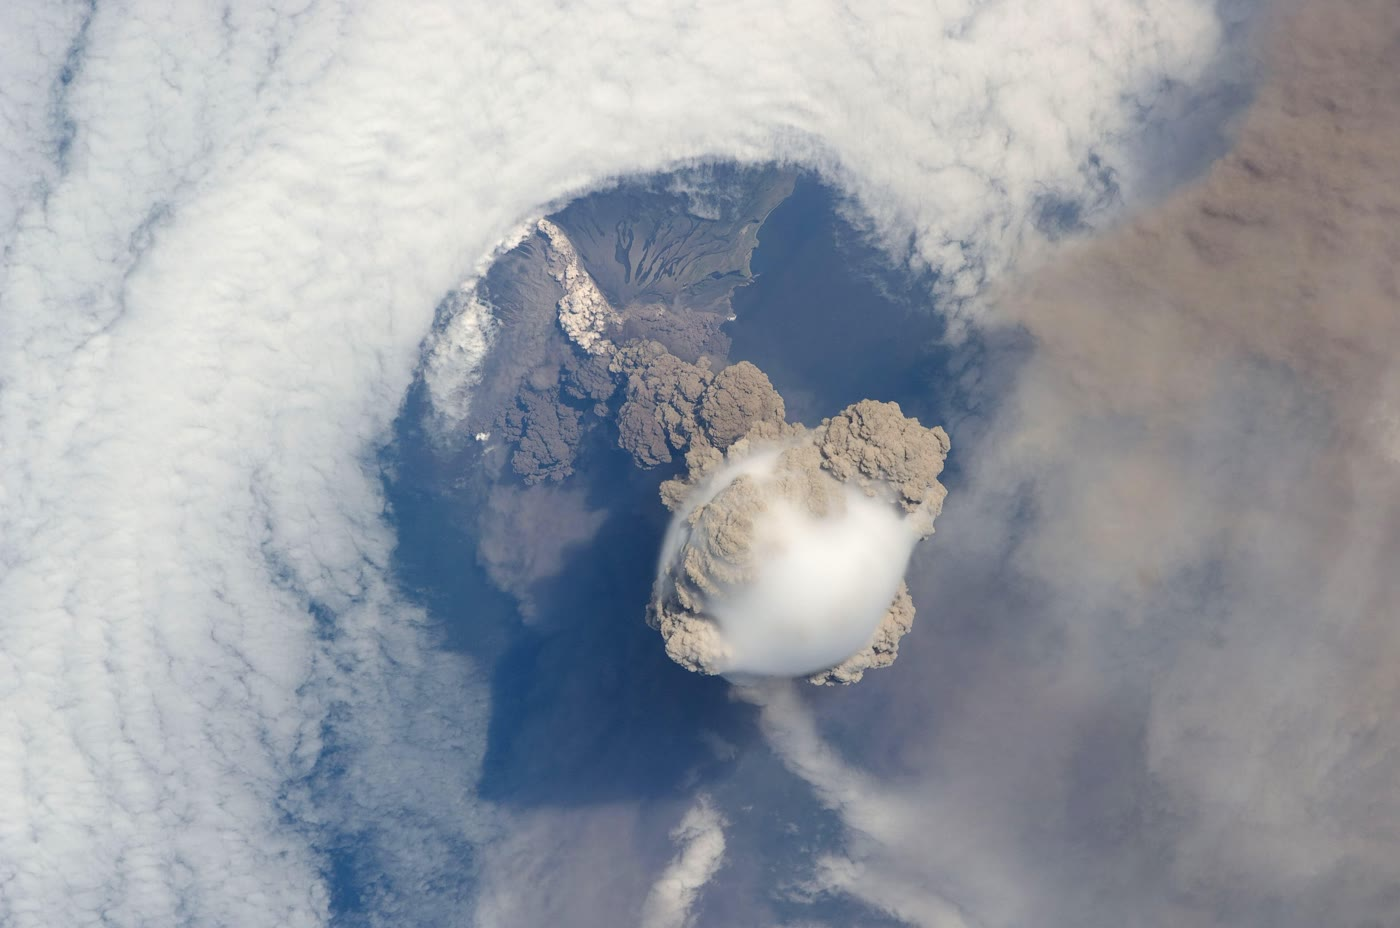
\includegraphics[width=0.66\linewidth]{images/book3/b1-sarychev-iss.jpg}
\par\smallskip{\small قمة سارتشيف، بركان من قوس كوريل على جزيرة ماتوا، في مرحلة مبكرة من ثوران في 12 يونيو 2009، منظورة من محطة الفضاء الدولية عبر ثقب في الغيوم. رماد رمادي، ربما تيار بيروكلاستي، ينحدر من القمة، وغطاء سحابي أملس يُسمّى البيليوس يجلس على العمود الصاعد؛ وقد رُصد رماد الثوران على بعد أكثر من \qty{2400}{km}. الصورة: NASA، ملك عام (Wikimedia Commons).}
\label{fig:b1:active-margins:sarychev}
\end{omfigure}
% ledger: nasa:sarychev, commons:sarychev

\omterm{def:b1:layered-earth:layers}{القشرة} تحت الأقواس تسمك بالتقصير وبالصهارة المضافة من الأسفل؛ وتحت الأقواس المبنية على القارات، مثل جبال الأنديز، تكون بين أسمك القشرات على الأرض.

وخلف بعض الأقواس تنشدّ الصفيحة المتراكبة. فسّر دان كاريغ أحواض الهوامش هذه في غرب المحيط الهادئ ضمن تكتونية الصفائح، عام 1971: فحين تغوص الكتلة بانحدار شديد وتتدحرج إلى الخلف، ينتقل الخندق والقوس نحو الصفيحة الغائصة، وتتمدّد الصفيحة التي خلفهما حتى تنشطر، فتترك أحيانًا قوسًا متبقيًا منقرضًا على الجانب البعيد. وفي نموذج الصفيحة المستعمل أعلاه، يبلغ انتشار خلف القوس نحو \qty{32}{mm.yr^{-1}} في حوض ماريانا قرب \ang{18}~ش، وأكثر من \qty{110}{mm.yr^{-1}} في شمال حوض لاو، خلف تونغا. أما حيث تكون الكتلة ضحلة، فعلى العكس، تسحب الصفيحة المتراكبة، فتُقصر قشرتها وتسمك خلف القوس، كما خلف الأنديز.
% ledger: karig:marginal-basins, data:pb2002 (ridge_budget.py: Mariana 32.4, Lau 117.5 mm/yr)

\begin{inthefield}[إنذار التسونامي]
لدى مركز إنذار التسونامي دقائق. ففي 2011 جاء أول إنذار لساحل شمال شرق اليابان بعد الزلزال بنحو ثلاث دقائق، استنادًا إلى قوة مبنية على الموجات الزلزالية قصيرة الدورة؛ ولزلازل قوتها 8 فأكثر تكون هذه القوة مقدّرة بأقل من حقيقتها، وكذلك كان ارتفاع التسونامي. أما قوة العزم، التي لا تتشبّع، فاستغرقت نحو خمس عشرة دقيقة: فمقاييس الزلازل ذات الحزمة العريضة في اليابان كانت قد تجاوزت مداها. ومنذ 2013، حين يكون حجم زلزال بهذا الكبر غير مؤكد، يفترض الإنذار الأول أكبر زلزال ممكن هناك، ويصف التسونامي بالكلمات، مثل «هائل»، لا بعدد؛ وتعتمد التنبؤات على قياسات البحر نفسه في عرض البحر، من عوامات محددة الموقع بالأقمار الصناعية ومقاييس ضغط على قاع البحر، تَرى الموجة قبل أن تصل الساحل.
% ledger: jma:warning

\smallskip
\begin{center}
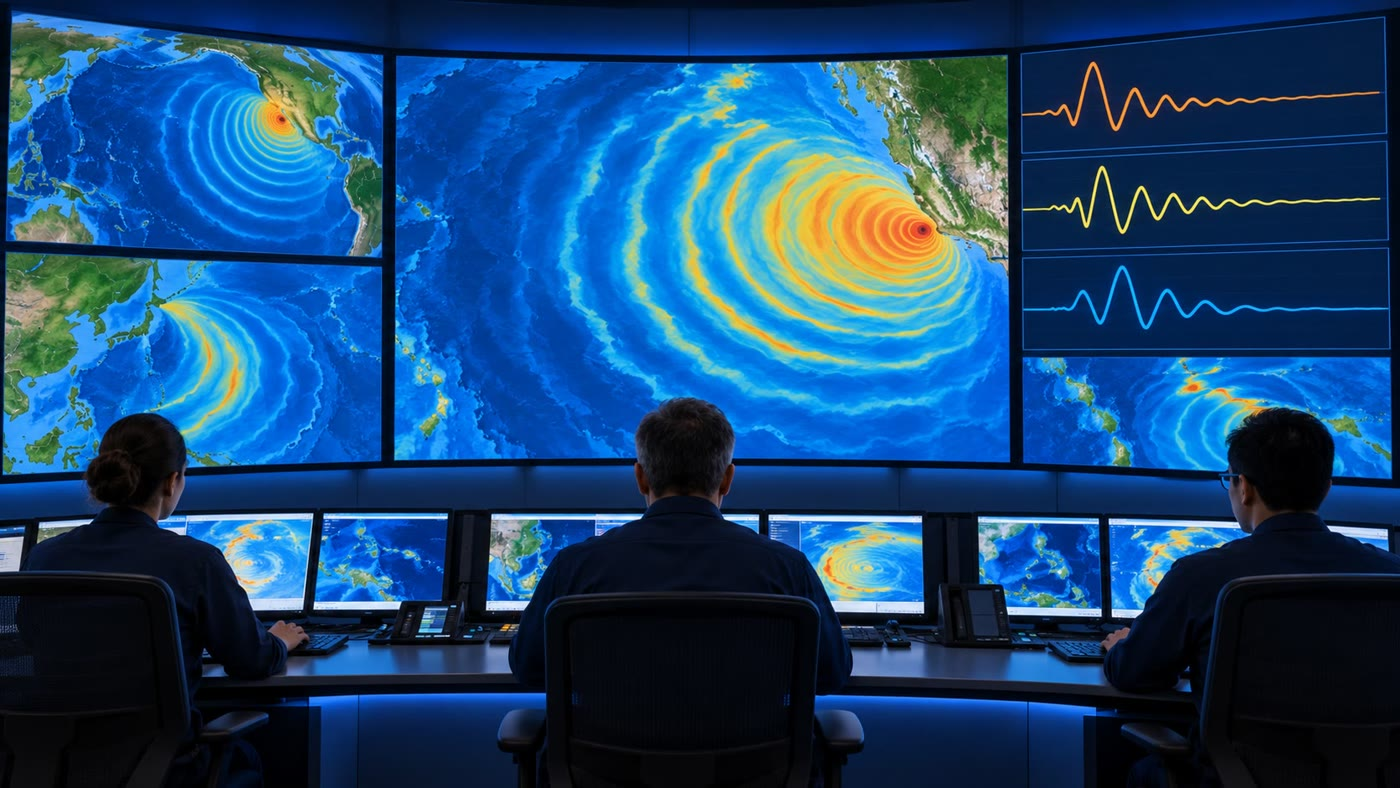
\includegraphics[width=0.7\linewidth]{images/book3/ai/b1-tsunami-centre.jpg}

{\scriptsize ضباط مناوبة في مركز إنذار التسونامي، أمام شاشات لجبهات الموجات المحسوبة وسجلات مستوى البحر (رسم توضيحي بالذكاء الاصطناعي).}
\end{center}
\end{inthefield}

\section{التمارين}

\begin{exercise}[$\star$]\label{exo:b1:active-margins:1}
يقع خندق \qty{3}{km} تحت قاع المحيط المحيط به. (أ) لو لم يُعوَّض، فبكم تخفض الصخرُ الغائبُ، كثافته \qty{2700}{kg.m^{-3}}، ويُستبدل بماء البحر كثافته \qty{1000}{kg.m^{-3}}، الجاذبيةَ هناك؟ استعمل صفيحة بوغيه، مع $G = \qty{6.674e-11}{m^3.kg^{-1}.s^{-2}}$. (ب) قارن بالشذوذ المرصود فوق خندق كوريل، نحو \qty{-260}{\milli\gal}، حيث يقع الخندق على \qty{3.5}{km} تحت القاع المحيط به: أعد الحساب لذلك العمق. (ج) لماذا يعطي الماء في خندق لا يتجاوز عرضه عشرات الكيلومترات أقل من صيغة الكتلة؟ وأين يجب أن يقع باقي العجز؟
\end{exercise}

\begin{exercise}[$\star$]\label{exo:b1:active-margins:2}
تدخل صفيحة المحيط الهادئ خندق كوريل بسرعة \qty{82}{mm.yr^{-1}}. (أ) ما طول الصفيحة الذي ينزل في 10 ملايين سنة؟ (ب) لو غاصت الكتلة على مسار مستقيم بانحدار \ang{45}، فكم سيكون عمق حافتها الأمامية حينئذٍ؟ (ج) كم يلزم حتى تبلغ \qty{600}{km}؟
\end{exercise}

\begin{exercise}[$\star$]\label{exo:b1:active-margins:3}
تقف البراكين فوق المكان الذي تكون فيه كتلة مستقيمة على عمق \qty{110}{km}. احسب \omterm{def:b1:active-margins:volcanic-arc}{فجوة القوس والخندق} لكتلة تنحدر بزاوية \ang{30} و\ang{45} و\ang{60}. أيّ قوس يقع أبعد عن خندقه؟
\end{exercise}

\begin{exercise}[$\star$]\label{exo:b1:active-margins:4}
في النموذج الرقمي للصفائح في الفصل، يندسّ نحو \qty{2.7}{km^2} من قاع المحيط عبر حدود الاندساس كل سنة، على طول نحو \qty{51000}{km}، وتتكوّن نحو \qty{3.0}{km^2} على طول نحو \qty{67000}{km} من حيود الانتشار. (أ) احسب متوسط معدّل التقارب ومتوسط \omterm{def:b1:plate-kinematics:spreading-rate}{معدّل الانتشار الكامل}، بوحدة \unit{mm.yr^{-1}}. (ب) عبر كل حدوده يفنى في النموذج من المساحة قدر ما يتكوّن. فأين يذهب باقي القاع الجديد؟
% ledger: data:pb2002 (ridge_budget.py: 2.739 km2 over 51471 km; 3.009 km2 over 67340 km; all 3.511 vs 3.519)
\end{exercise}

\begin{exercise}[$\star\star$]\label{exo:b1:active-margins:5}
أربعة زلازل لمقطع تقع عند $(x, z) = (200, 150)$ و$(300, 250)$ و$(400, 330)$ و$(500, 430)$، بالكيلومتر. (أ) ركّب خط الكتلة بالمربعات الصغرى، وأعطِ انحداره. (ب) أين يبلغ الخط السطح؟ (ج) قارن بانحدار الخط المار بالزلزالين الأول والأخير وحدهما.
\end{exercise}

\begin{exercise}[$\star\star$]\label{exo:b1:active-margins:6}
كتلة نموذجية تنحدر بزاوية \ang{25} من الخندق حتى \qty{50}{km}، ثم بزاوية \ang{45}. وتقف الجبهة البركانية فوق المكان الذي تكون فيه الكتلة على عمق \qty{110}{km}. (أ) احسب \omterm{def:b1:active-margins:volcanic-arc}{فجوة القوس والخندق}. (ب) قارن بكتلة تنحدر بزاوية \ang{45} على امتدادها كله. (ج) إذا مُدّ القطاع العميق صعودًا، فأين يبلغ السطح؟ قارنه بخط كوريل، الذي يبلغ السطح على بعد \qty{53}{km} نحو اليابسة من الخندق. (د) ما الفجوة التي يعطيها قطاع عميق بانحدار \ang{60}؟
\end{exercise}

\begin{exercise}[$\star\star$]\label{exo:b1:active-margins:7}
(أ) وفق قضية القشرة المنحنية، ما نصف القطر الزاوي، وما نصف القطر بالكيلومترات ($R = \qty{6371}{km}$)، الذي ينبغي أن يكون للقوس فوق كتلة تنحدر بزاوية \ang{45}؟ \ang{30}؟ \ang{70}؟ (ب) أيّ الأقواس أشدّ انحناءً؟ (ج) الكتلة الكورية تنحدر بزاوية \ang{44.9}، ودائرة خندق كوريل تطابق دائرةً بقياس \ang{21.9}: احسب الفرق النسبي عن التنبؤ.
\end{exercise}

\begin{exercise}[$\star\star$]\label{exo:b1:active-margins:8}
خذ ناقلية قدرها \qty{2.5}{W.m^{-1}.K^{-1}} وحرارة سطح قدرها \qty{10}{\celsius}. (أ) احسب تدرّج حرارة السطح تحت منطقة أمامية تفقد \qty{35}{mW.m^{-2}}، وتحت \omterm{def:b1:active-margins:active-margin}{حوض خلف القوس} الذي يفقد \qty{80}{mW.m^{-2}}. (ب) إذا مدّدت هذين التدرجين خطيًا، فقدّر الحرارة عند \qty{30}{km} في كل منهما. (ج) تُقاس موهوات أحواض خلف القوس عند 800 إلى \qty{900}{\celsius}. لماذا يكون التقدير الخطي مرتفعًا أكثر من اللازم؟
% ledger: hyndman:backarc (back-arc 70-85, Moho 800-900); the forearc value is an exercise value
\end{exercise}

\begin{exercise}[$\star\star$]\label{exo:b1:active-margins:9}
في نموذج الصفيحة المستعمل في الفصل، ينفتح حوض ماريانا قرب \ang{18}~ش بمعدّل كامل نحو \qty{32}{mm.yr^{-1}}. (أ) عبّر عن هذا المعدّل بوحدة \unit{km.Myr^{-1}}، وأعطِ المعدّل النصفي إذا كان الانتشار متماثلًا. (ب) كم يلزم للحوض حتى ينفتح بمقدار \qty{100}{km} بهذا المعدّل؟ (ج) أعطِ سببين يمنعان قراءة عمر \omterm{def:b1:active-margins:active-margin}{حوض خلف القوس} ببساطة من عرضه ومعدّله الحالي.
% ledger: data:pb2002 (ridge_budget.py: mariana_18n_mm_yr 32.4)
\end{exercise}

\begin{exercise}[$\star\star\star$]\label{exo:b1:active-margins:10}
كتلة سمكها \qty{100}{km} تغوص بسرعة \qty{82}{mm.yr^{-1}} على مسار ينحدر بزاوية \ang{45}. خذ $\kappa = \qty{e-6}{m^2.s^{-1}}$. (أ) كم يلزم لتبلغ \qty{600}{km}؟ (ب) إلى أي مدى تنتشر الحرارة داخلها في تلك المدة، بحساب $\sqrt{\kappa t}$؟ (ج) كم يلزم للحرارة لتبلغ منتصفها؟ (د) استنتج عن حرارة الكتلة عند \qty{600}{km}، وعن زلازلها.
\end{exercise}

\begin{exercise}[$\star\star\star$]\label{exo:b1:active-margins:11}
\omterm{def:b1:active-margins:accretionary}{لكومة تراكمية} نموذجية مقطع مثلثي: سطحها ينحدر بزاوية $\alpha = \ang{4}$ نحو الخندق، وقاعدتها تنحدر بزاوية $\beta = \ang{6}$ تحتها، ويلتقيان عند طرفها؛ وتحتفظ بهاتين الزاويتين وهي تنمو. (أ) أثبت أن مساحتها $A = \frac12 L^2(\tan\alpha + \tan\beta)$ من أجل عرض $L$، عندما تكون الزوايا صغيرة بما يكفي ليكون الارتفاع عند الخلف $L(\tan\alpha + \tan\beta)$. (ب) تصل رواسب سمكها \qty{1}{km} إلى صفيحة تتقارب بسرعة \qty{40}{mm.yr^{-1}}، وتُكشط كلها: احسب العرض بعد 1 و\num{4} و\num{10} ملايين سنة. كيف ينمو $L$ مع الزمن؟ (ج) ماذا لو هبط نصف الرواسب مع الكتلة؟
\end{exercise}

\begin{exercise}[$\star\star\star$]\label{exo:b1:active-margins:12}
(أ) أثبت أن خط المربعات الصغرى يمرّ بالنقطة المتوسطة $(\bar x, \bar z)$. (ب) يسجّل كتالوج كل عمق أعمق بمقدار \qty{10}{km} من الحقيقي. كيف يتغيّر ميل الخط المركَّب وقطعه؟ (ج) تُقاس المسافات $x$ كلها من نقطة خندق وُضعت أبعد نحو اليابسة بمقدار \qty{20}{km}، فكل $x$ أصغر بمقدار \qty{20}{km}. كيف يتغيّر الميل والقطع؟ (د) هل يغيّر أيّ من الخطأين \omterm{def:b1:geological-maps:attitude}{الانحدار}؟
\end{exercise}

\section{مسألة: قراءة منطقة اندساس من زلازلها}

\begin{problem}[{مسألة نهاية الأسبوع: الكتلة الكورية من ثمانية زلازل، وسرعة هبوطها، وما تقوله جاذبيتها وتدفّقها الحراري، وأين ينبغي أن تقف براكينها}]
\label{pb:b1:active-margins:1}
% values: calc/ch14.py; the eight events are real (USGS catalogue, rounded to the km)
% from figdata/out/bachelor-1-slab_seismicity-section.dat
% ledger: data:b3-usgs-kuril, data:pb2002, data:b2-seafloor-age, syracuse:arc-depth, frank:arcs,
% data:b3-grav-kuril, parsons:plate-model, hyndman:backarc; the forearc heat flow is an exercise value
ثمانية زلازل من الكتلة الكورية، كلها أعمق من \qty{70}{km}، مُدرجة بحسب مسافتها $x$ من الخندق على خط المقطع، نحو بحر أوخوتسك، وعمقها $z$، مُقرّبتين إلى الكيلومتر.

\begin{center}
\small
\begin{tabular}{lcccccccc}
\hline
الحدث & \mbox{\textdir TLT 1} & \mbox{\textdir TLT 2} & \mbox{\textdir TLT 3} & \mbox{\textdir TLT 4} & \mbox{\textdir TLT 5} & \mbox{\textdir TLT 6} & \mbox{\textdir TLT 7} & \mbox{\textdir TLT 8}\\
$x$ (\unit{km}) & \mbox{\textdir TLT 155} & \mbox{\textdir TLT 222} & \mbox{\textdir TLT 305} & \mbox{\textdir TLT 319} & \mbox{\textdir TLT 431} & \mbox{\textdir TLT 533} & \mbox{\textdir TLT 578} & \mbox{\textdir TLT 609}\\
$z$ (\unit{km}) & \mbox{\textdir TLT 96} & \mbox{\textdir TLT 169} & \mbox{\textdir TLT 245} & \mbox{\textdir TLT 272} & \mbox{\textdir TLT 389} & \mbox{\textdir TLT 489} & \mbox{\textdir TLT 518} & \mbox{\textdir TLT 573}\\
القوة & \mbox{\textdir TLT 5.5} & \mbox{\textdir TLT 5.1} & \mbox{\textdir TLT 5.0} & \mbox{\textdir TLT 5.4} & \mbox{\textdir TLT 5.3} & \mbox{\textdir TLT 5.3} & \mbox{\textdir TLT 5.2} & \mbox{\textdir TLT 6.4}\\
\hline
\end{tabular}
\end{center}

\medskip
\noindent\textbf{الجزء الأول --- خط الكتلة.}
\begin{enumerate}
  \item ارسم الزلازل الثمانية بالمقياس نفسه على المحورين، والعمق نحو الأسفل.
  \item احسب $\sum x_i$ و$\sum z_i$ و$\sum x_i^2$ و$\sum x_i z_i$، والمتوسطين $\bar x$ و$\bar z$.
  \item احسب $S_{xx}$ و$S_{xz}$، ثم ميل خط المربعات الصغرى إلى ثلاث منازل عشرية، وقطعه إلى منزلة عشرية واحدة.
  \item ما انحدار الكتلة؟
  \item أين يبلغ الخط السطح؟ ماذا يقول ذلك عن شكل الكتلة قرب الخندق؟
  \item احسب الانحراف $z_i - (a + s x_i)$ لكل زلزال. أيّها أبعد عن الخط، وبكم؟
\end{enumerate}

\medskip
\noindent\textbf{الجزء الثاني --- كم تهبط الكتلة بسرعة.} عند بداية المقطع يعطي نموذج PB2002 تقاربًا قدره \qty{87.4}{mm.yr^{-1}}: بالنسبة إلى صفيحة أوخوتسك، تتحرك صفيحة المحيط الهادئ نحو \omterm{def:b1:spherical-astronomy:horizontal}{السمت} \ang{300}. ويمتد خط المقطع، العمودي على الخندق، نحو \omterm{def:b1:spherical-astronomy:horizontal}{السمت} \ang{320.9}.
\begin{enumerate}[resume]
  \item احسب الزاوية بين التقارب وخط المقطع، ثم مركبتي التقارب العمودية على الخندق والموازية له.
  \item ما طول الصفيحة الذي ينزل عبر الخندق في 10 ملايين سنة؟
  \item باستعمال انحدار السؤال 4 (مقرّبًا إلى \ang{45})، كم يلزم للكتلة لتحمل نقطة من أعلاها من الخندق إلى أعمق زلزال في الشريط، \qty{632}{km}؟ أهمل \omterm{def:b1:geological-maps:attitude}{الانحدار} الأخفّ قرب الخندق.
  \item الصفيحة عمرها نحو \qty{122}{Myr} عند الخندق. ما عمر قاع البحر الذي يقع الآن على عمق \qty{632}{km}؟
  \item بحساب $\sqrt{\kappa t}$، مع $\kappa = \qty{e-6}{m^2.s^{-1}}$، إلى أي مدى تنتشر الحرارة في الكتلة خلال ذلك الهبوط؟ قارنه بسمكها، نحو \qty{100}{km}.
\end{enumerate}

\medskip
\noindent\textbf{الجزء الثالث --- الجاذبية والتدفّق الحراري.} خذ ناقلية قدرها \qty{2.5}{W.m^{-1}.K^{-1}}.
\begin{enumerate}[resume]
  \item يفقد قاع المحيط القديم أمام الخندق نحو \qty{43}{mW.m^{-2}}، \omterm{def:b1:active-margins:active-margin}{وحوض خلف القوس} نحو \qty{80}{mW.m^{-2}}؛ وخذ \qty{35}{mW.m^{-2}} للمنطقة الأمامية. احسب تدرّج الحرارة قرب السطح لكلٍّ منها.
  \item فسّر لماذا تفقد المنطقة الأمامية حرارة أقل من قاع المحيط القديم أمامها.
  \item \omterm{def:b1:isostasy-gravity:anomalies}{شذوذ الهواء الحر} فوق خندق كوريل نحو \qty{-260}{\milli\gal}. ما سماكة الصخر الذي يفوق كثافته كثافة الماء بمقدار \qty{1700}{kg.m^{-3}}، التي تحتاجها صفيحة بوغيه لتعطي هذا العجز؟ قارنها بعمق الخندق تحت القاع المحيط به، نحو \qty{3.5}{km}.
  \item لنفترض الآن أن الصفيحة كلها هُبطت بمقدار \qty{3.5}{km}: يحلّ الماء محلّ الصخر في أعلاها، وتحلّ \omterm{def:b1:layered-earth:layers}{القشرة} محلّ \omterm{def:b1:layered-earth:layers}{الوشاح} في قاعدتها، فيحلّ الماء، في المجموع، محلّ \omterm{def:b1:layered-earth:layers}{وشاح} كثافته \qty{3300}{kg.m^{-3}}. احسب شذوذ صفيحة بوغيه. لماذا يعطي الخندق الحقيقي، الذي لا يتجاوز عرضه عشرات الكيلومترات، أقل من ذلك؟
  \item الخندق والرفعة الخارجية ليسا في توازن أيزوستاتي. ما الذي يبقيهما خارجه؟
\end{enumerate}

\noindent\textbf{الجزء الرابع --- أين ينبغي أن تقف البراكين.} استعمل الخط الوارد في السؤال 3، مع ميله وقطعه المقرّبين.
\begin{enumerate}[resume]
  \item أول بركان في الشريط يبعد \qty{164}{km} عن الخندق. على أي عمق تقع الكتلة تحته؟
  \item هل هذا العمق ضمن المدى الذي يوجد تحت الأقواس، من 72 إلى \qty{173}{km}؟ وكم يبعد عن المتوسط، \qty{105}{km}؟
  \item على أي بُعد من الخندق تكون الكتلة على عمق \qty{100}{km}؟
  \item وفق قضية القشرة المنحنية، ما نصف القطر الزاوي الذي ينبغي أن يكون لقوس كوريل، وما نصف القطر بالكيلومترات؟
  \item يطابق خندق كوريل \omterm{def:b1:spherical-astronomy:spherical-triangle}{دائرة صغرى} بقياس \ang{21.9}. قارِن.
  \item تقف البراكين القوسية، في المتوسط، حيث تكون الكتلة على عمق نحو \qty{105}{km}. على أي بُعد من الخندق يبلغ خط الكتلة هذا العمق؟
  \item قارن هذه المسافة بالمسافة المرصودة \qty{164}{km}: بكم كيلومترًا، وبأي كسر تختلف؟
  \item بأقرب كيلومتر، ما \omterm{def:b1:active-margins:volcanic-arc}{فجوة القوس والخندق} التي يتنبأ بها خط الكتلة الكورية للبراكين الواقفة فوق الكتلة على \qty{105}{km}؟
\end{enumerate}
\end{problem}
